\chapter{Differences to Project Plan}
\label{chapter:differences}

This chapter gives an overview of the differences between the scheduled and effective needed time of our workpackages based on the \textit{Project Plan (Figure 3) in Project Manual}.

\section{Work Package: Initialization}
\begin{table}[H]
\begin{center}
  \begin{tabular}{|l|l|l|l|}
    \hline
      \multicolumn{2}{|>{\columncolor[gray]{0.82}}p{3.85in}|}{\bfseries{\textsf{Work Package: Initialization}}} \\
    \hline
      \multicolumn{1}{|p{2.5in}|}{\bfseries{\textsf{Time Scheduled}}} &
      \multicolumn{1}{|p{1in}|}{9 Days} \\
      \multicolumn{1}{|p{2.5in}|}{\bfseries{\textsf{Effective Time}}} &
      \multicolumn{1}{|p{1in}|}{9 Days} \\
    \hline \hline
      \multicolumn{1}{|p{2.5in}|}{\bfseries{\textsf{Difference}}} &
      \multicolumn{1}{|p{1in}|}{0 Days} \\
    \hline
  \end{tabular}
\end{center}
\caption{Workpackage Initialization}
\end{table}

\section{Work Package: Concept}
\begin{table}[H]
\begin{center}
  \begin{tabular}{|l|l|l|l|}
    \hline
      \multicolumn{2}{|>{\columncolor[gray]{0.82}}p{3.85in}|}{\bfseries{\textsf{Work Package: Concept}}} \\
    \hline
      \multicolumn{1}{|p{2.5in}|}{\bfseries{\textsf{Time Scheduled}}} &
      \multicolumn{1}{|p{1in}|}{15 Days} \\
      \multicolumn{1}{|p{2.5in}|}{\bfseries{\textsf{Effective Time}}} &
      \multicolumn{1}{|p{1in}|}{15 Days} \\
    \hline \hline
      \multicolumn{1}{|p{2.5in}|}{\bfseries{\textsf{Difference}}} &
      \multicolumn{1}{|p{1in}|}{0 Days} \\
    \hline
  \end{tabular}
\end{center}
\caption{Workpackage Concept}
\end{table}

\section{Work Package: Collaboration 1}
\begin{table}[H]
\begin{center}
  \begin{tabular}{|l|l|l|l|}
    \hline
      \multicolumn{2}{|>{\columncolor[gray]{0.82}}p{3.85in}|}{\bfseries{\textsf{Work Package: Collaboration 1}}} \\
    \hline
      \multicolumn{1}{|p{2.5in}|}{\bfseries{\textsf{Time Scheduled}}} &
      \multicolumn{1}{|p{1in}|}{8 Days} \\
      \multicolumn{1}{|p{2.5in}|}{\bfseries{\textsf{Effective Time}}} &
      \multicolumn{1}{|p{1in}|}{8 Days} \\
    \hline \hline
      \multicolumn{1}{|p{2.5in}|}{\bfseries{\textsf{Difference}}} &
      \multicolumn{1}{|p{1in}|}{0 Days} \\
    \hline
  \end{tabular}
\end{center}
\caption{Workpackage Collaboration 1}
\end{table}

\section{Work Package: GUI 1}
\begin{table}[H]
\begin{center}
  \begin{tabular}{|l|l|l|l|}
    \hline
      \multicolumn{2}{|>{\columncolor[gray]{0.82}}p{3.85in}|}{\bfseries{\textsf{Work Package: GUI 1}}} \\
    \hline
      \multicolumn{1}{|p{2.5in}|}{\bfseries{\textsf{Time Scheduled}}} &
      \multicolumn{1}{|p{1in}|}{8 Days} \\
      \multicolumn{1}{|p{2.5in}|}{\bfseries{\textsf{Effective Time}}} &
      \multicolumn{1}{|p{1in}|}{8 Days} \\
    \hline \hline
      \multicolumn{1}{|p{2.5in}|}{\bfseries{\textsf{Difference}}} &
      \multicolumn{1}{|p{1in}|}{0 Days} \\
    \hline
  \end{tabular}
\end{center}
\caption{Workpackage GUI 1}
\end{table}

\section{Work Package: Network 1}
\begin{table}[H]
\begin{center}
  \begin{tabular}{|l|l|l|l|}
    \hline
      \multicolumn{2}{|>{\columncolor[gray]{0.82}}p{3.85in}|}{\bfseries{\textsf{Work Package: Network 1}}} \\
    \hline
      \multicolumn{1}{|p{2.5in}|}{\bfseries{\textsf{Time Scheduled}}} &
      \multicolumn{1}{|p{1in}|}{8 Days} \\
      \multicolumn{1}{|p{2.5in}|}{\bfseries{\textsf{Effective Time}}} &
      \multicolumn{1}{|p{1in}|}{8 Days} \\
    \hline \hline
      \multicolumn{1}{|p{2.5in}|}{\bfseries{\textsf{Difference}}} &
      \multicolumn{1}{|p{1in}|}{0 Days} \\
    \hline
  \end{tabular}
\end{center}
\caption{Workpackage Network 1}
\end{table}

\section{Work Package: Merge 1}
The first merge of the three layers caused more problems than excepted. Some problems with merging the different branches together and some minor incompatibilities between the layers leaded to the delay of two days.
\begin{table}[H]
\begin{center}
  \begin{tabular}{|l|l|l|l|}
    \hline
      \multicolumn{2}{|>{\columncolor[gray]{0.82}}p{3.85in}|}{\bfseries{\textsf{Work Package: Merge 1}}} \\
    \hline
      \multicolumn{1}{|p{2.5in}|}{\bfseries{\textsf{Time Scheduled}}} &
      \multicolumn{1}{|p{1in}|}{6 Days} \\
      \multicolumn{1}{|p{2.5in}|}{\bfseries{\textsf{Effective Time}}} &
      \multicolumn{1}{|p{1in}|}{8 Days} \\
    \hline \hline
      \multicolumn{1}{|p{2.5in}|}{\bfseries{\textsf{Difference}}} &
      \multicolumn{1}{|p{1in}|}{+2 Days} \\
    \hline
  \end{tabular}
\end{center}
\caption{Workpackage Merge 1}
\end{table}

\section{Work Package: Documentation 1}
To spare some time for the development we decided to reduce this block of explizit writing documentation. To compensate that, everyone documented besides the following implementation work packages.
\begin{table}[H]
\begin{center}
  \begin{tabular}{|l|l|l|l|}
    \hline
      \multicolumn{2}{|>{\columncolor[gray]{0.82}}p{3.85in}|}{\bfseries{\textsf{Work Package: Documentation 1}}} \\
    \hline
      \multicolumn{1}{|p{2.5in}|}{\bfseries{\textsf{Time Scheduled}}} &
      \multicolumn{1}{|p{1in}|}{6 Days} \\
      \multicolumn{1}{|p{2.5in}|}{\bfseries{\textsf{Effective Time}}} &
      \multicolumn{1}{|p{1in}|}{4 Days} \\
    \hline \hline
      \multicolumn{1}{|p{2.5in}|}{\bfseries{\textsf{Difference}}} &
      \multicolumn{1}{|p{1in}|}{-2 Days} \\
    \hline
  \end{tabular}
\end{center}
\caption{Workpackage Documentation 1}
\end{table}

\section{Work Package: Collaboration 2}
This workpackage was originaly not planned, but due upcoming changes (e.g. simple access management and some minor changes) in the framework we had to spend more time to the collaboration layer.
\begin{table}[H]
\begin{center}
  \begin{tabular}{|l|l|l|l|}
    \hline
      \multicolumn{2}{|>{\columncolor[gray]{0.82}}p{3.85in}|}{\bfseries{\textsf{Work Package: Collaboration 2}}} \\
    \hline
      \multicolumn{1}{|p{2.5in}|}{\bfseries{\textsf{Time Scheduled}}} &
      \multicolumn{1}{|p{1in}|}{0 Days} \\
      \multicolumn{1}{|p{2.5in}|}{\bfseries{\textsf{Effective Time}}} &
      \multicolumn{1}{|p{1in}|}{4 Days} \\
    \hline \hline
      \multicolumn{1}{|p{2.5in}|}{\bfseries{\textsf{Difference}}} &
      \multicolumn{1}{|p{1in}|}{+4 Days} \\
    \hline
  \end{tabular}
\end{center}
\caption{Workpackage Collaboration 2}
\end{table}

\section{Work Package: GUI 2}
The choose of good frameworks and the prototypes made before the diploma work, leaded to a faster development of the GUI.
\begin{table}[H]
\begin{center}
  \begin{tabular}{|l|l|l|l|}
    \hline
      \multicolumn{2}{|>{\columncolor[gray]{0.82}}p{3.85in}|}{\bfseries{\textsf{Work Package: GUI 2}}} \\
    \hline
      \multicolumn{1}{|p{2.5in}|}{\bfseries{\textsf{Time Scheduled}}} &
      \multicolumn{1}{|p{1in}|}{12 Days} \\
      \multicolumn{1}{|p{2.5in}|}{\bfseries{\textsf{Effective Time}}} &
      \multicolumn{1}{|p{1in}|}{9 Days} \\
    \hline \hline
      \multicolumn{1}{|p{2.5in}|}{\bfseries{\textsf{Difference}}} &
      \multicolumn{1}{|p{1in}|}{-3 Days} \\
    \hline
  \end{tabular}
\end{center}
\caption{Workpackage GUI 2}
\end{table}

\section{Work Package: Network 2}
Some annoying problems occured in the network layer (more or less known bugs in the \textit{beep core} library) made the delaying of this workpackages.
\begin{table}[H]
\begin{center}
  \begin{tabular}{|l|l|l|l|}
    \hline
      \multicolumn{2}{|>{\columncolor[gray]{0.82}}p{3.85in}|}{\bfseries{\textsf{Work Package: Network 2}}} \\
    \hline
      \multicolumn{1}{|p{2.5in}|}{\bfseries{\textsf{Time Scheduled}}} &
      \multicolumn{1}{|p{1in}|}{12 Days} \\
      \multicolumn{1}{|p{2.5in}|}{\bfseries{\textsf{Effective Time}}} &
      \multicolumn{1}{|p{1in}|}{15 Days} \\
    \hline \hline
      \multicolumn{1}{|p{2.5in}|}{\bfseries{\textsf{Difference}}} &
      \multicolumn{1}{|p{1in}|}{+3 Days} \\
    \hline
  \end{tabular}
\end{center}
\caption{Workpackage Network 2}
\end{table}

\section{Work Package: Merge 2}
We excepted more problems in the second merge phase and thus we planned to spend more time to this package. Finaly this work package needed less time but had a delay of approximate three days (because of the network layer problems).
\begin{table}[H]
\begin{center}
  \begin{tabular}{|l|l|l|l|}
    \hline
      \multicolumn{2}{|>{\columncolor[gray]{0.82}}p{3.85in}|}{\bfseries{\textsf{Work Package: Merge 2}}} \\
    \hline
      \multicolumn{1}{|p{2.5in}|}{\bfseries{\textsf{Time Scheduled}}} &
      \multicolumn{1}{|p{1in}|}{6 Days} \\
      \multicolumn{1}{|p{2.5in}|}{\bfseries{\textsf{Effective Time}}} &
      \multicolumn{1}{|p{1in}|}{4.5 Days} \\
    \hline \hline
      \multicolumn{1}{|p{2.5in}|}{\bfseries{\textsf{Difference}}} &
      \multicolumn{1}{|p{1in}|}{-1.5 Days} \\
    \hline
  \end{tabular}
\end{center}
\caption{Workpackage Merge 2}
\end{table}

\section{Work Package: Stabilization}
After the good progress from the work package \textit{Merge 2} and the good test results we needed less time to realize a stable version of ACE.
\begin{table}[H]
\begin{center}
  \begin{tabular}{|l|l|l|l|}
    \hline
      \multicolumn{2}{|>{\columncolor[gray]{0.82}}p{3.85in}|}{\bfseries{\textsf{Work Package: Stabilization}}} \\
    \hline
      \multicolumn{1}{|p{2.5in}|}{\bfseries{\textsf{Time Scheduled}}} &
      \multicolumn{1}{|p{1in}|}{7.5 Days} \\
      \multicolumn{1}{|p{2.5in}|}{\bfseries{\textsf{Effective Time}}} &
      \multicolumn{1}{|p{1in}|}{5 Days} \\
    \hline \hline
      \multicolumn{1}{|p{2.5in}|}{\bfseries{\textsf{Difference}}} &
      \multicolumn{1}{|p{1in}|}{-2.5 Days} \\
    \hline
  \end{tabular}
\end{center}
\caption{Workpackage Stabilization}
\end{table}

\section{Work Package: Documentation 2}
\begin{table}[H]
\begin{center}
  \begin{tabular}{|l|l|l|l|}
    \hline
      \multicolumn{2}{|>{\columncolor[gray]{0.82}}p{3.85in}|}{\bfseries{\textsf{Work Package:  Documentation 2}}} \\
    \hline
      \multicolumn{1}{|p{2.5in}|}{\bfseries{\textsf{Time Scheduled}}} &
      \multicolumn{1}{|p{1in}|}{16.5 Days} \\
      \multicolumn{1}{|p{2.5in}|}{\bfseries{\textsf{Effective Time}}} &
      \multicolumn{1}{|p{1in}|}{16.5 Days} \\
    \hline \hline
      \multicolumn{1}{|p{2.5in}|}{\bfseries{\textsf{Difference}}} &
      \multicolumn{1}{|p{1in}|}{0 Days} \\
    \hline
  \end{tabular}
\end{center}
\caption{Workpackage Documentation 2}
\end{table}

\section{Work Package: Close Down}
\begin{table}[H]
\begin{center}
  \begin{tabular}{|l|l|l|l|}
    \hline
      \multicolumn{2}{|>{\columncolor[gray]{0.82}}p{3.85in}|}{\bfseries{\textsf{Work Package:  Close Down}}} \\
    \hline
      \multicolumn{1}{|p{2.5in}|}{\bfseries{\textsf{Time Scheduled}}} &
      \multicolumn{1}{|p{1in}|}{6 Days} \\
      \multicolumn{1}{|p{2.5in}|}{\bfseries{\textsf{Effective Time}}} &
      \multicolumn{1}{|p{1in}|}{6 Days} \\
    \hline \hline
      \multicolumn{1}{|p{2.5in}|}{\bfseries{\textsf{Difference}}} &
      \multicolumn{1}{|p{1in}|}{0 Days} \\
    \hline
  \end{tabular}
\end{center}
\caption{Workpackage Close Down}
\end{table}

\section{Corrected Project Plan}
In the \emph{Project Manual} a project plan can be found. Now, here we show
you the reality. The differences have been explained before:

\begin{figure}[H]
 \centering
 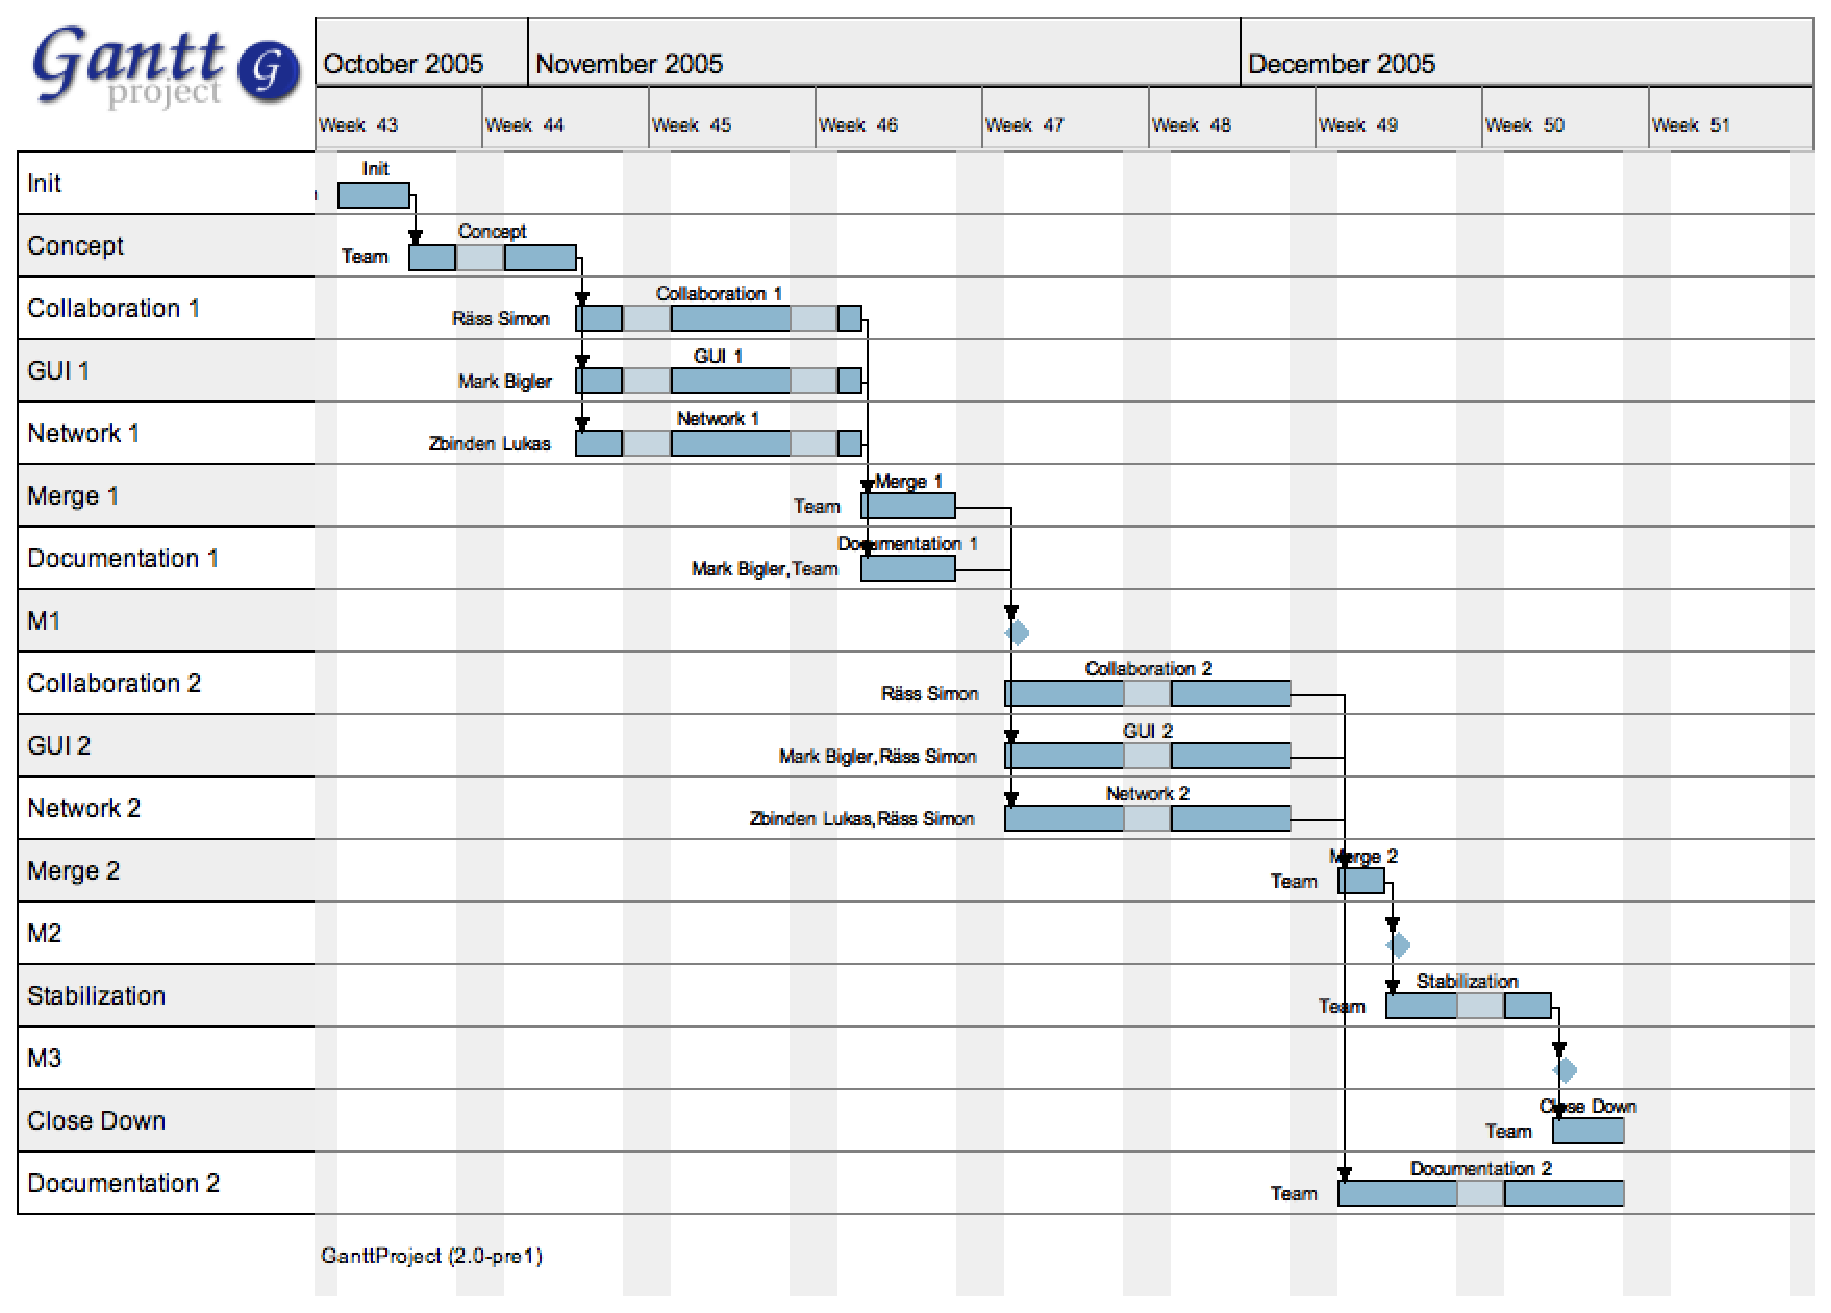
\includegraphics[width=20cm,width=14.27cm,angle=90]{../images/finalreport/projectplan/ace.eps}
 \caption{Corrected Project Plan (Reality)}
\end{figure}

